\chapter{Eulerian Graphs}

\section{Relevant Definitions}

\begin{definition}[Walks]
  A \textit{walk} in a graph is a sequence of the form \(v_1, e_1, v_2, e_2,
  ..., v_r\) for some \(r \geq 1\) where \(v_i\)'s are vertices and
  \(e_i\)'s are edges from \(v_i \to v_{i+1}\) for each \(1 \leq i < r\).
\end{definition}

\begin{remark}
  General walks can have repeated edges and/or vertices. In addition, if 
  \(r = 1\), then the walk consists of a single vertex and no edge.
\end{remark}

\begin{definition}[Trails]
  A \textit{trail} is a walk with no repeated edges.
\end{definition}

\begin{definition}[Circuits]
  A \textit{circuit} is a closed trail. That is, it is a walk that starts and
  ends on the same vertex with no repeated edges.
\end{definition}

\begin{definition}[Path Alt.]
  A \textit{path} is a trail in which no vertex appears more than once. That is,
  it is a walk with no repeated vertices nor edges.
\end{definition}

\section{Eulerian Graphs}

\begin{definition}[Eulerian Graphs]
  A connected graph \(G\) is \textit{Eulerian} if there exists a circuit containing
  every edge of \(G\). This is also known as an \textit{Eulerian Circuit}.
\end{definition}

\begin{definition}[Semi-Eulerian Graphs]
  A non-Eulerian graph \(G\) is \textit{semi-Eulerian} if there exists an open trail
  containing every edge of \(G\). This trail is also known as an 
  \textit{Eulerian Trail}.
\end{definition}

\begin{figure}[ht]
  \begin{center}
    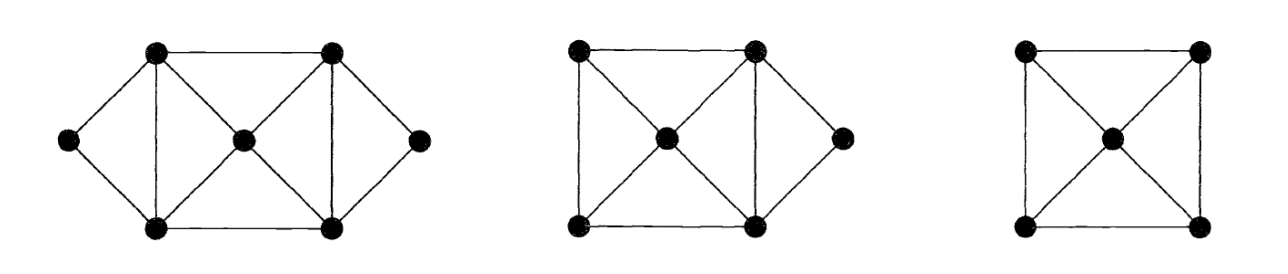
\includegraphics[width=0.69\textwidth]{figures/l02/eulerian-graphs}
  \end{center}
  \caption{(Left to right) Eulerian, semi-Eulerian, and non-Eulerian graphs}\label{fig:eulerian-graphs}
\end{figure}

\begin{theorem}[Euler, 1736]
  A connected graph \(G\) is Eulerian if and only if the degree of each vertex 
  of \(G\) is even.
\end{theorem}

\begin{proof}
  Disclaimer: This proof follows what is shown in the lecture and a YouTube video \cite{euler-graph-prf}.

  First, we will show the forward case: If a connected graph \(G\) is Eulerian---that is, if \(G\) has an Eulerian circuit in \(G\)---then the degree of each vertex is even. Suppose that \(P\) is an Euler circuit. Whenever \(P\) passes through a vertex (except for the start and end vertices), it contributes 2 edges to said vertex. Since each edge occurs exactly once in the trail, each vertex must have an even degree.

  Next, we will show the converse case: If every vertex of a connected graph \(G\) has an even degree, then \(G\) is Eulerian. Consider the trail of maximum length, denoted \(T\). First, we will show that \(T\) is a circuit. Suppose that \(T\) starts at vertex \(v\) and ends at \(w\). If \(v = w\), then we are done. Otherwise, we consider the end vertex \(w\). \(w\) may have already been visited in \(T\), each time also visiting two edges---one to enter and one to leave. Consequently, we have an extra edge going into \(w\), making its degree odd. For \(w\) to have an even degree, there must be another vertex \(u\) not yet visited in \(T\). However, if there is an edge to \(u\), then we are extending the maximum trail---a contradiction. Hence, we have that \(T\) is a circuit in \(G\). 

  Now, we claim that \(E(T) = E(G)\). Assume to the contrary that \(E(T) \subsetneq E(G)\). Then, there must be an edge \(e = (x, y)\) of \(G\) that is not in \(E(T)\) but is incident to \(x \in V(T)\). Let us consider the subgraph \(H\) such that \(E(H) = E(G) \setminus E(T)\). Notice that when a vertex shows up in \(T\), it is incident to two edges in \(T\). Thus, removing \(E(T)\) from \(E(G)\) removes an even number of edges from each vertex in \(T\). Since the vertices of \(H\) are vertices of \(G\) which have even degrees, removing even edges from each vertex results in every vertex in \(H\) having an even degree as well. Without loss of generality, assume that \(H\) is connected. If not, the same reasoning can be applied to each component of \(H\). Consider the trail of maximum length in \(H\) that starts from \(x\), denoted \(T'\). Then, using the same reasoning as before, we have that \(T'\) is a circuit of \(H\) starting from \(x\). We can recursively apply this procedure until we run out of edges in \(G\). 

  Finally, we can construct a circuit \(C\) by inserting \(T'\) into \(T\) when we arrive at \(x\) in \(T\). However, this is a contradiction since we are extending a maximum-length circuit \(T\). Hence, we have that \(T\) is already a circuit that visits every vertex in \(G\). Therefore, we can conclude that if every vertex of a connected graph \(G\) has an even degree, then \(G\) is Eulerian.
  % That is, we want to show that it is possible to construct an Eulerian Circuit that visits every edge of \(G\). The construction are as follows:
  % \begin{enumerate}
  %   \item Since every vertex in \(G\) has an even degree, each edge must have at
  %     least 2 adjacent vertices. In addition, since \(G\) is connected, we are
  %     able to identify a cycle, say \(C\). 
  %   \item Remove the edges of \(C\) from \(G\) and call this subgraph \(H\).
  %     Note that \(H\) may be disconnected. 
  %   \item For each component of \(H\), claim that every vertex in \(H\) also has
  %     an even degree. Repeat this until all the edges are visited by a cycle. 
  %   \item To finally construct the Euler Cirtcuit of \(G\), we trace the edges
  %     of the cycle \(C\). If we reach 
  % \end{enumerate}
\end{proof}

\section{Fleury's Algorithm}


